\documentclass[12pt]{article}

\usepackage{geometry}
\geometry{a4paper}

%% \usepackage[active,tightpage]{preview}
%% \PreviewEnvironment{eqnarray}
%% \PreviewEnvironment{equation}



%\textwidth = 290pt

\usepackage{graphicx}
\usepackage{float}
\usepackage{wrapfig}

\linespread{1.2} % Line spacing

\graphicspath{{figs/}}

\usepackage{polski}
\usepackage[utf8]{inputenc}

\DeclareFixedFont{\ttb}{T1}{txtt}{bx}{n}{12} % for bold
\DeclareFixedFont{\ttm}{T1}{txtt}{m}{n}{12}  % for normal
\usepackage{color}
\definecolor{deepblue}{rgb}{0,0,0.5}
\definecolor{deepred}{rgb}{0.6,0,0}
\definecolor{deepgreen}{rgb}{0,0.5,0}
\usepackage{listings}


% Python style for highlighting
\newcommand\pythonstyle{\lstset{
language=Python,
basicstyle=\ttm,
otherkeywords={self},             % Add keywords here
keywordstyle=\ttb\color{deepblue},
emph={MyClass,__init__},          % Custom highlighting
emphstyle=\ttb\color{deepred},    % Custom highlighting style
stringstyle=\color{deepgreen},
frame=tb,                         % Any extra options here
showstringspaces=false            %
}}
% Python environment
\lstnewenvironment{python}[1][]
{
\pythonstyle
\lstset{#1}
}
{}
% Python for external files
\newcommand\pythonexternal[2][]{{
\pythonstyle

\lstinputlisting[#1]{#2}}}
% Python for inline
\newcommand\pythoninline[1]{{\pythonstyle\lstinline!#1!}}

\title{Proste modele ze złożonym zachowaniem \\ czyli o chaosie}
\begin{document}
\maketitle
\lstset{language=Python}


{\em Komputer jest narzędziem coraz częściej stosowanym przez naukowców do
ukazywania skrzętnie ukrywanych przez naturę tajemnic. Symulacja, obok
eksperymentu i teorii, staje się trzecim sposobem badania świata. }


Na Uniwersytecie Śląskim trzy lata temu rozpoczęliśmy program
integracji metod komputerowych z edukacją. W efekcie powstało wiele
niezwykle fascynujących materiałów dydaktycznych pozwalających na
łatwiejsze i bardziej dogłębne poznanie wielu tematów. Jako podstawowe
narzędzie został wybrany język Python, który wraz z potęgą dostępnych
w nim bibliotek naukowych, stanowi obecnie chyba najlepsze rozwiązanie
do ``komputerowego eksperymentowania'' z równaniami, obrazami czy
danymi. Jedną z ciekawszych implementacji kompletnego środowiska pracy
jest program Sage\cite{sagemath}. Stanowi on otwartą integrację
systemu algebry komputerowej z językiem Python, ponadto umożliwia
rozpoczęcie zabawy od zaraz, korzystając z przeglądarki internetowej i
jednej z możliwych opcji dostępu poprzez usługę chmurową\cite{cloud}
lub server pojedyńczych obliczeń, na którym bazuje interaktywna wersja
tego artykułu\cite{web}.



\section{Chaos w ekologii}

W latach siedemdziesiątych XX wieku na Uniwersytecie w Oxford
australijski uczony Robert May zajmował się teoretycznymi aspektami
dynamiki populacyjnej. Swoje prace podsumował w artykule, który ukazał
się w \emph{Nature} pod prowokującym tytułem ``Proste modele
matematyczne z bardzo skomplikowaną dynamiką'' \cite{may76}. Artykuł
ten po latach stał się jedną z najczęściej cytowanych prac z
teoretycznej ekologii. Co wzbudziło tak wielkie zainteresowanie w tej
pracy?

Klasycznym zadaniem dynamiki populacyjnej jest obliczenie populacji
pewnego gatunku w przyszłości znając jego obecny stan. Matematycznie
najprostszym rodzajem ekosystemów wydawały się takie, w których życie
jednego pokolenia populacji trwa jeden sezon. Dobrym przykładem jest
populacja owadów, które w ciągu jednego sezonu przechodzą pełną
metamorfozę, np. motyle. Czas jest w naturalny sposób podzielony na
dyskretne\footnote{W matematyce ``dyskretny'' to przyjmujący wartości
  z określonego przeliczalnego zbioru. Przeciwieństwem jest
  ``ciągły''} okresy, odpowiadające cyklom życia populacji. Równania
opisujące taki ekosystem mają więc w naturalny sposób tzw. dyskretny
czas, tj. $t=1,2,3...$. Robert May zajmował się między innymi właśnie
taką dynamiką. W swoich rozważaniach uprościł ekosystem do jednego
gatunku, w którym populacja była funkcją kwadratową populacji w roku
poprzednim. Skąd taki model?

Najprostszym równaniem dyskretnym opisującym ewolucję populacji jest
model liniowy:

\begin{equation}
\label{eq:Ni}
N_{i+1} = \alpha \; N_{i},
\end{equation}
%
gdzie $N_i$ to liczebność w i-tym sezonie, a $N_{i+1}$ opisuje
populację w następnym sezonie. Łatwo się przekonać, że takie równanie
może prowadzić to trzech scenariuszy.  Dla $\alpha=1$ ewolucja nie
będzie zmieniać stanu liczebnego populacji, $\alpha<1$ prowadzi do
wyginięcia, a przypadek $\alpha>1$ oznacza nieograniczony wzrost
populacji. To prowadziłoby do zachwiania równowagi w
przyrodzie. Ponieważ wszystko w przyrodzie jest ograniczone, warto
poprawić to równanie w taki sposób aby brało pod uwagę ograniczoną
ilość zasobów. Wyobraźmy sobie, że szkodniki zjadają zboże, którego
jest dokładnie ta sama ilość co roku. Jeżeli owadów jest mało w
porównaniu do ilości pożywienia to mogą rozmnażać się z pełną siła
rozrodczą matematycznie określoną przez stałą $\alpha>1$. Jednak w
miarę wzrostu liczebności szkodników, pożywienia nie będzie wystarczać
i siła rozrodcza będzie maleć. W krytycznym przypadku można sobie
wyobrazić ze owadów rodzi się tyle, że zjadają całe zboże przed
osiągnięciem zdolności rozrodczej i populacja ginie.  Model
uwzględniający ten efekt ograniczonego dostępu do pożywienia został po
raz pierwszy zaproponowany przez Verhulsta w roku 1838. W modelu tym
tempo wzrostu $\alpha$ nie jest stałe, ale zależy od stanu populacji:
%
\begin{equation}
\label{eq:V}
\alpha = \alpha( N_{i} )
\end{equation}
%
Zależność tempa wzrostu $\alpha$ od $N_i$ powinna mieć następującą
własność: jeżeli populacja wzrasta, tempo wzrostu powinno maleć
ponieważ jest utrudniony dostęp do pożywienia. Oczywiście jest wiele
funkcji o tej własności: to są funkcje malejące. Verhulst zaproponował
taką oto zależność:
%
\begin{equation}
\label{eq:V1}
\alpha = a \left(1-\frac{N_{i}}{K} \right)
\end{equation}
%
gdzie $a>0$ oraz stała $K>0$ charakteryzuje zasoby pożywienia i nazywa
sie pojemnością środowiska. Jak zmiana K wpływa na tempo wzrostu
populacji? Jeżeli K rośnie to $N_i/K$ maleje. Z kolei to powoduje że
$1-N_i/K$ rośnie, czyli $\alpha$ rośnie. Oznacza to, że tempo wzrostu
rośnie i populacja rozrasta się szybciej.  Zmodyfikujmy więc poprzedni
model (\ref{eq:Ni}) zakładając, że tempo wzrostu $\alpha$ zmienia się
tak jak w równaniu (\ref{eq:V1}). Wówczas otrzymamy równanie
%
\begin{equation}
\label{eq:N2i}
N_{i+1} = a \left(1-\frac{N_{i}}{K} \right) \; N_{i}
\end{equation}
%
Równanie to można zapisać w postaci równania rekurencyjnego
%
\begin{equation}
x_{i+1} = a x_{i} (1 - x_{i}),
\label{eq:logistic}
\end{equation}
%
gdzie $x_i = N_i/K$ oraz $x_{i+1} = N_{i+1}/K$ oznaczają przeskalowane
liczebności populacji w czasie $i$ oraz w czasie $i+1$. Równanie (\ref{eq:logistic})
nazywa się {\em równaniem logistycznym}.

Mogłoby się wydawać, że przy tak niewielkiej modyfikacji nasz model
jest prosty do analizy. Sprawdźmy to. Rozważmy równanie
(\ref{eq:logistic}) dla parametru $a=0.5$ startując z początkowej
populacji $x_0=0.45$. Kolejne wartości populacji można otrzymać
stosując równanie rekurencyjne (\ref{eq:logistic}):
%
\begin{eqnarray}
x_{1} &=& a x_{0} (1 - x_{0}), \nonumber \\
x_{2} &=& a x_{1} (1 - x_{1}), \nonumber \\
x_{3} &=& a x_{2} (1 - x_{2}), \quad \mbox{itd}
\end{eqnarray}
 
%
Aby ułatwić obliczenia w (6) możemy skorzystać z poniższego
programu\footnote{Program jest napisany w języku Python i można go
  uruchomić m.in. na platformie Sage. Zachęcamy do lektury książki
  http://icse.us.edu.pl/e-book/} symulującego nasz model:

\pythonexternal{code01.py}

Obliczamy kolejne wartości $x_i$ i zauważamy, że maleją one do zera.
Eksperymentując z powyższym kodem łatwo też jest się przekonać, że
dzieję się tak od wartości początkowej $x_0$. Oznacza to, że populacja
zawsze ginie.

W drugim kroku analizy zwiększamy wartość parametru $a$ do dowolnej
wartości z przedziału $a\in(1,3)$.  Okazuje się, że wtedy ciąg $x_i$
dąży do pewnej wielkości $x^{*}>0$. Interpretując to w kategoriach
ekologii możemy powiedzieć, że wielkość populacji ustala się na pewnym
poziomie, który nie zmienia się z sezonu na sezon. Warto zauważyć, że
wartość $x^*$ nie zależy od stanu początkowego $x_0$. Jest to efekt
dążenia ekosystemu do stabilizacji - populacja dostosowuje swoją
liczebność do możliwości wyżywienia się. Matematycznie mówimy, że
układ dąży do stabilnego punktu stałego, tj. spełniającego równość
$x^{*}=f(x^{*})$ (oznacza to że w chwili następnej stan jest taki sam
jak w chwili poprzedniej). Z pomocą programu Sage możemy przedstawić
tę ewolucję graficzne rysując wykres liczebności populacji od czasu.
%
\begin{figure}
    \begin{center}
     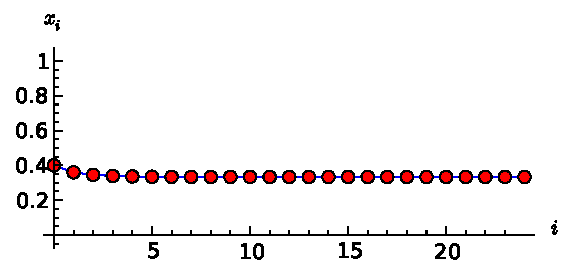
\includegraphics{xi1.pdf}
  \end{center}
  \caption{Dla  $a=1.5$ ekosystem osiąga dynamiczną równowagę.
    \label{fig:a1} }
\end{figure}
%

Taki efekt stabilizacji był oczekiwany przez badaczy i równanie
logistyczne (\ref{eq:logistic}) nie przyciągnęłoby szczególnej uwagi
gdyby nie pewna niespodzianka. Okazało się bowiem, że dla pewnych
wartości parametru $a$ model (\ref{eq:logistic}) nie zachowuje się w
przewidywalny sposób. Po pierwsze, pojawiają się stany okresowe i
wielo-okresowe. Po drugie, z każdym krokiem czasowym populacja zmienia
się w nieregularny sposób, podobny do losowego ruchu. Po trzecie,
pojawia się duża wrażliwość na warunki początkowe: dwa prawie
nierozróżnialne warunki początkowe prowadzą do całkowicie różnej
ewolucji populacji. Wszystkie te cechy są charakterystyczne dla
zachowania które przypomina ruch całkowicie losowy i nazywa się {\em
  deterministycznym chaosem}.

Zbadajmy tę własność! 
\begin{figure}
  \begin{center}
    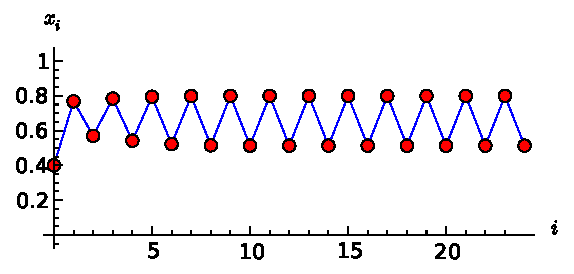
\includegraphics{xi2.pdf}
    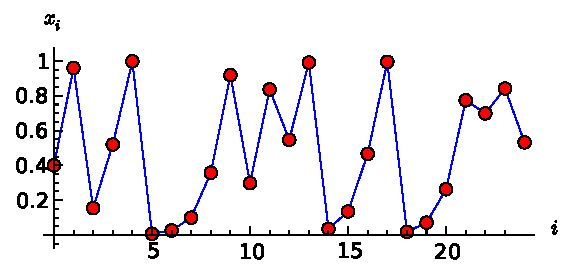
\includegraphics{xi3.pdf}
  \end{center}
 \caption{Dla $a=3.2$ (góra) ewolucja układu prowadzi to oscylacji. W
   tym przypadku populacja co drugi sezon jest taka sama. Dla $a=4$
   (dół) liczba osobników w kolejnych latach zdaje się być losowa!
 \label{fig:a34} }
\end{figure}
%

Na początek ustalmy wartość parametru na $a = 3.2$ i przyjrzyjmy się
ewolucji. Zaskoczeniem może być fakt, że tym razem populacja nie
osiąga jednej wartości, ale dwie, które występują kolejno po sobie co
drugi sezon.  Okazało się jednak, że to nie koniec kłopotów.
Dla $a=4$ układ przestaje być przewidywalny. Popatrzmy na rysunek
(\ref{fig:a34}) lub wygenerujmy sami ciąg liczb za pomocą
komputera. Wyniki wyglądają na czysto przypadkowe i dla nieco
różniących się populacji początkowych są kompletnie różne. Uważny
czytelnik powinien jednak zaprotestować. Jak układ, który jest opisany
przez deterministyczne\footnote{Prawo deterministyczne to takie w
  którym przyszłość jest jednoznacznie określona przez stan
  początkowy. Antonimem jest prawo probablistyczne.} równanie, do tego
nawet całkiem proste, może mieć nieprzewidywalne zachowanie?  Otóż
może. Własnością tego układu jest niezwykła czułość na warunki
początkowe. Wystarczy wystartować z dwóch warunków początkowych
różniących się o jedną milionową i już po kilku krokach otrzymamy
całkiem inne wartości populacji. Sprawdźmy to przy pomocy komputera:

\pythonexternal{code02.py}

Oto mamy prosty model deterministycznej ewolucji. Ale ten determinizm
jest złudny, jest determinizmem tylko matematycznym. Z praktycznego
punktu widzenie układ zachowuje się w sposób nieprzewidywalny ponieważ
nigdy nie możemy zadać warunków początkowych w matematycznie dokładny
sposób. W rzeczywistości wszystko jest określane z pewną dokładnością:
każdy przyrząd pomiarowy ma określoną dokładność i to może być
przyczyną praktycznej nieprzewidywalności w deterministycznych
układach posiadających własność chaotyczności. Przykładem niech będą
modele prognozy pogody które zawsze wykazują własność
chaotyczności. Dlatego tak kiepskie bywają prognozy pogody w dłuższym
przedziale czasowym.

Analiza układów chaotycznych jest niezwykle trudna. Możemy jednak dość
łatwo odkryć wiele tajemnic chaotyczności stosując symulacje
komputerowe. Narysujmy tak zwany diagram bifurkacyjny, na którym
będziemy odkładać na osi odciętych wartości parametru $a$ a na osi
rzędnych stabilne punkty stałe odwzorowania logistycznego. Stabilne
punkty otrzymamy symulując dużą ilość układów jednocześnie i rysując
wartości po wieku krokach obliczeń. Jak można się domyślić wymaga to
wykonania dużej ilości obliczeń. Spróbujmy ``ostrożnie'' postępować z
następującymi wartościami:

\pythonexternal{code03.py}

Powinniśmy otrzymać coś podobnego do rysunku (\ref{fig:bd}). Jak
interpretować ten rysunek?  Np. dla wartości parametru $a=3.3$ mamy 2
stabilne punkty stałe (co drugi sezon populacja ma tą samą
liczebność). Np. dla parametru $a=3.5$ mamy 4 punkty stałe (co czwarty
sezon populacja ma tą samą liczebność). Np. dla parametru $a=3.56$
mamy 8 punktów stałych (co ósmy sezon populacja ma tą samą
liczebność). Ale dla parametru $a\approx 3.57$ mamy nieskończenie
wiele punktów stałych (liczebność w populacji nigdy się nie powtarza i
zmienia się w nieprzewidywalny sposób).  Mając jednak program
komputerowy, możemy zmienić zakres parametru $a$ i eksplorować
własnoręcznie niekończącą się strukturę geometryczną owego diagramu.
\begin{figure} % Inline image example
  \begin{center}

    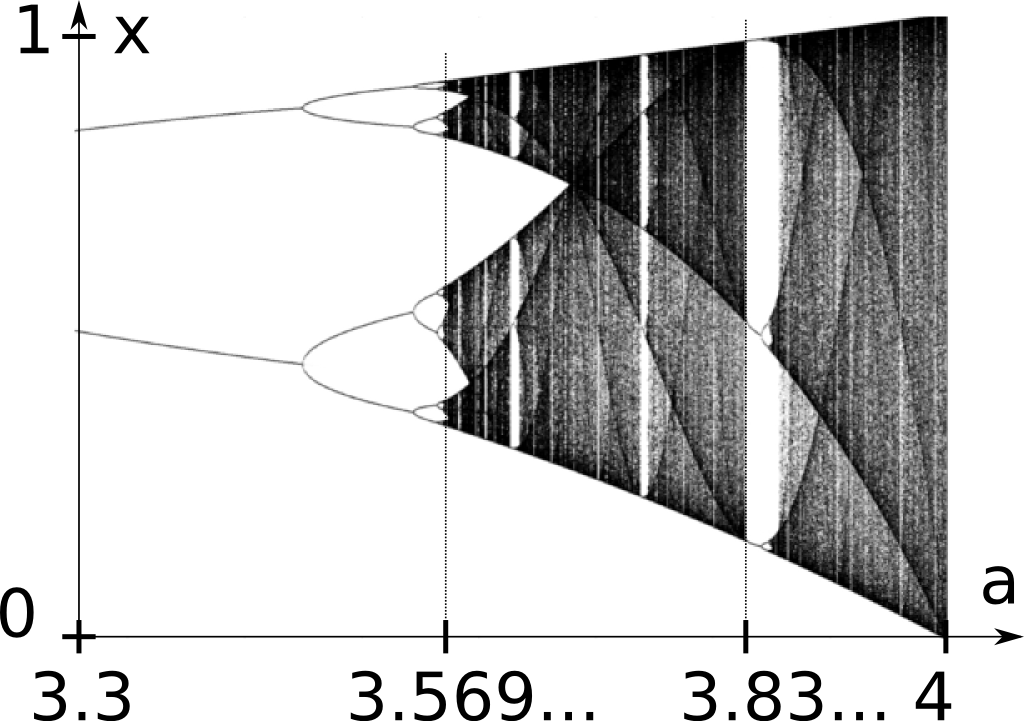
\includegraphics[width=0.8\linewidth]{Bifurcation_diagram.png}
  \end{center}
  \caption{Diagram bifurkacyjny dla równania logistycznego    \label{fig:bd} }
\end{figure}
To tylko czubek góry lodowej. Na temat tego równania napisano tysiące
prac naukowych i mimo tego wciąż skrywa ono swoje tajemnice. Z pomocą
symulacji komputerowej można, nawet bez stosowania zaawansowanej
matematyki pobawić się w odkrywcę świata dynamiki
nieliniowej. Zapraszamy do lektury wersji online, zawierającej
szczegóły wielu ciekawych własności równania logistycznego oraz
interesujące sposoby ich wizualizacji.

\begin{thebibliography}{1}
\bibitem{may76}
May, R. M. ``Simple mathematical models with very complicated dynamics''. Nature 261 (5560): 459–467,1976.

\bibitem{sagemath} http://sagemath.org
\bibitem{cloud} http://cloud.sagemath.com
\bibitem{web} http://visual.icse.us.edu.pl/Warsztaty

\end{thebibliography}

\end{document}

%sagemathcloud={"zoom_width":110}
